% !TeX spellcheck = en_US
\newpage
\section{Link}
\subsection{NIC}
The \textbf{Network Interface Card} is a piece of hardware that provides link layer abstraction to the device network's stack. They are of two types:
\begin{itemize}
	\item \textbf{Point-to-point}: high bandwidth bidirectional links, with a dedicated channel per direction thus avoiding collisions
	\item \textbf{Broadcast}: medium shared in a way that creates collisions if more devices transmit at the same time
\end{itemize}

\subsection{Framing}
Messages are organized in \textbf{frames}, well defined structures, as follows:
\begin{center}
	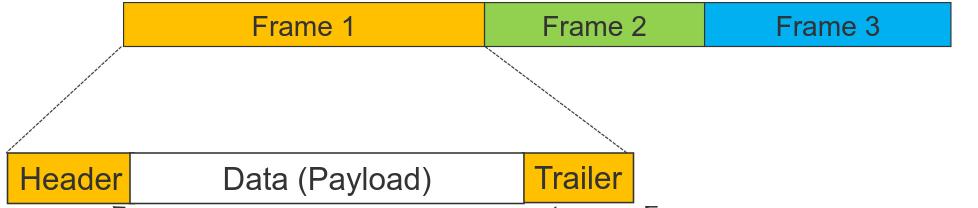
\includegraphics[scale=0.25]{frame}
\end{center}
\begin{itemize}
	\item \textbf{Preamble}: before the header, flag byte sequence marking the beginning of a frame and sometimes the frame length
	\item \textbf{Header}: control information (e.g. addresses, frame numbers)
	\item \textbf{Error check}: inside the Trailer, contains \textbf{Frame Checking Sequence}
	\item \textbf{Postamble}: after the Trailer, flag byte sequence marking end of a frame
\end{itemize}

\subsubsection{Character count} 
A good addition is using the first value to advertise the number of characters in the frame, thus eliminating the \textit{Postamble}.
\begin{center}
	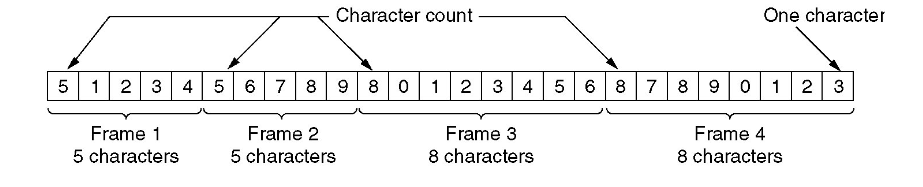
\includegraphics[scale=0.3]{charcount}
\end{center}

\subsubsection{Character stuffing}
Start and end of a frame are represented by a special byte sequence. Since the flag byte may occur in the payload, \textbf{character} stuffing is done: a special escape byte \textit{ESC} is inserted by the sender and then removed by the receiver. The escape byte may also appear in the payload and thus it may also be stuffed itself.
\begin{center}
	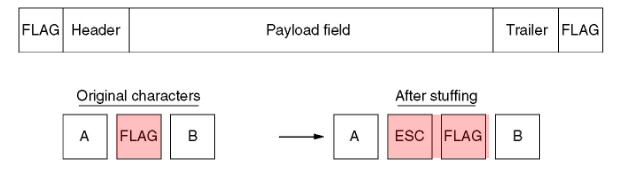
\includegraphics[scale=0.3]{charstuff}
\end{center}
The generic version is the \textbf{bit stuffing}: inserting a $0$ after five consecutive $1$.

\subsubsection{Physical layer}
Framing can also exploit special symbols from the physical layer:
\begin{itemize}
	\item \textbf{4B5B}: use the special symbols as control characters
	\item \textbf{PHY coding violations}: in Manchester code no mid-bit edge can appear, therefore the start and end of a frame can be coded as a violation of that rule
\end{itemize}

\subsection{Error detection and correction}
Transmissions over the physical layer are not error free. Hence, error \textbf{detection} and \textbf{correction }is necessary. The solution is to add \textbf{error control data} to each frame: a frame of $m$ bits receives $r$ check bits, creating a \textbf{codeword} of $n=m+r$ bits.

\subsubsection{Frame Check Sequence}
A very naive solution is to repeat the payload and then do a bit-wise comparison. It's very effective but has a huge \textbf{overhead}.

\paragraph{Parity bit}
This technique reduces the overhead by counting the number of $1$ in the payload and setting the \textbf{parity bit} to $1$ if there is an \textbf{even} amount of them. This adds a $1$bit overhead only but doesn't check for \textit{even} errors and doesn't allow correction.

\paragraph{Double parity}
Group bits together to form a matrix and then compute parity bits for each row and column. Compared to single parity, can identify more errors (not all) and correct some of them.
\begin{center}
	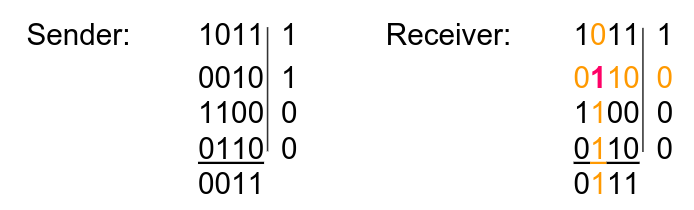
\includegraphics[scale=0.3]{doublepar}
\end{center}

\paragraph{Modulo check}
Parity bits don't handle well error \textbf{bursts\footnote{Group of errors close together, very frequent in data communication.}}. Modulo check tries to solve this by computing a frame check sequence based on a modulo operation: interprets the payload as a number $N$ and appends a control integer $C$ such that
\begin{equation*}
	(N + C) \% 11 = 0
\end{equation*}
Bit errors are detected by recomputing the modulo at the receiver end.
\begin{center}
	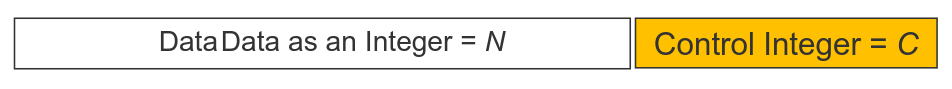
\includegraphics[scale=0.3]{modulo}
\end{center}
The generic version is the \textbf{Cyclic Code Checksum}, which allows you to choose the number of bits dedicated to the checksum and the base of the modulo, extremely lowering the probability of undetected errors (if tuned correctly).

\paragraph{Cyclic Redundancy Checksum}
A payload of $m$ bit $a_{m-1}, \ldots, a_0$ is seen as a \textbf{polynomial} $a_{m-1}x^{m-1} + \ldots + a_0$. The sender and the receiver then agree on a \textbf{generator polynomial}
\begin{equation*}
	G(x) = g_r x^r + g_{r-1} x^{r-1} + \ldots + g_1 x^1 + g_0 x^0 \qquad\qquad g_r = g_0 = 1
\end{equation*}
The sender then interprets a data block of length $m$ as a polynomial 
\begin{equation*}
	M(x) = a_{m-1}x^{m-1} + \ldots + a_1x^1 + a_0x^0
\end{equation*}
and adds redundant bits so that the extended polynomial $M'(x)$ is divisible by $G(x)$.
\begin{lstlisting}[mathescape=true]
	r = degree(generator_polynomial)
	extended_data_bits = data_bits + (r zeros)  // Concatenate r zeros
	remainder_bits = binary_division(extended_data_bits, generator_polynomial)
	checksummed_frame = extended_data_bits XOR remainder_bits
\end{lstlisting}
On the other hand the receiver divides the received extended polynomial $M'(x)$ by $G(x)$ and if the remainder is $0$ then no error occurred.\\
CRC will detect all error bursts of length $\leq r$. It \textbf{will not recognize} if instead of $T(x)$, $T(x)+E(x)$ with $E(x)$ containing $G(x)$ as a factor.
\begin{note}
	Common 16-bit generators are:
	\begin{itemize}
		\item \textbf{CRC-16} $G(x) = x^{16} + x^{15} + x^2 +1$
		\item \textbf{CRC CITT} $G(x) = x^{16} + x^{12} + x^5 + 1$
		\item \textbf{Ethernet} $G(x) = x^32 + x^{26} + x^{23} + x^{22} + x^{16} + x^{12} + x^{11} + x^{10} + x^8 + x^7 + x^5 + x^4 +x^2 + x+1$
	\end{itemize}
\end{note}
The \textbf{hardware} implementation for CRC uses \textbf{shift registers} with XOR for subtraction and AND for applying it.
\begin{example}
	Circuit for the generator polynomial
	\begin{equation*}
		G(x) = x^4 + x + 1
	\end{equation*}
	\begin{center}
		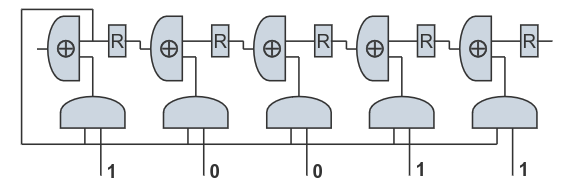
\includegraphics[scale=0.4]{crc}
	\end{center}
\end{example}

\subsubsection{Hamming Distance}
The Hamming Distance is the number of places in which two binary sequences differ. Given an $m$bit long \textbf{data} with $2^m$ possible \textit{data words}, $r$ \textbf{check bits} and thus $n=m+r$ bit \textbf{codewords}, build a list of all the possible $2^n$ codewords and find the two with the minimum distance. This allows to:
\begin{itemize}
	\item \textbf{Detect} $d$ errors, having a distance of at least $d+1$
	\item \textbf{Correct} $d$ errors, having a distance of at least $2d+1$
\end{itemize}

\begin{example}
	Given a code with only two possible codewords:
	\begin{align*}
		& w_1=000 \\
		& w_2 = 111
	\end{align*}
	We have a distance of $3$, meaning we can \textbf{detect} $2$ bits errors and correct $1$bit ones:
	\begin{itemize}
		\item $001$ received, we can correct it
		\item $110$ received, cannot be recovered
	\end{itemize}
\end{example}

While the Hamming Code can correctly identify and correct $1$bit errors, it's expensive in terms of required check bits and can't correct $2$bits errors and cannot identify $3$bits ones.

\subsubsection{Correction mechanism}
\paragraph{Forward Error Correction} Uses error correcting codes (RS, BCH): they can be corrected in most cases, \textbf{discarded} otherwise. It's low latency since the feedback from the receiver to the sender is not needed, therefore suitable for \textbf{delay sensitive} transmissions.

\paragraph{Automatic Repeat reQuest}
Uses error-detecting codes (CRC): if data contains errors, it needs to be sent again from the sender. Suitable for \textbf{error sensitive} transmissions. Using ARQ means managing the \textbf{control flow} (numbering data blocks, receipt acknowledgment, retransmission).

\subsection{Flow control}
Let's define a sketch of the interface between the Link layer and the Network and Physical layers.
\begin{lstlisting}[language=C]
	#define MAX_PKT 1024 /* determines packet size in bytes */
	
	typedef enum {false, true} boolean; /* boolean type */
	
	typedef unsigned int seq_nr; /* sequence or ack numbers */
	
	typedef struct {
		unsigned char data[MAX_PKT];
	} packet; /* packet definition */
	
	typedef enum {data, ack, nak} frame_kind; /* kinds of frames */
	
	typedef struct { /* frames are transported in this layer */
		frame_type type; /* what kind of a frame is it? */
		seq_nr seq; /* sequence number */
		seq_nr ack; /* acknowledgement number */
		packet info; /* the network layer packet */
	} frame;
\end{lstlisting}
\begin{center}
	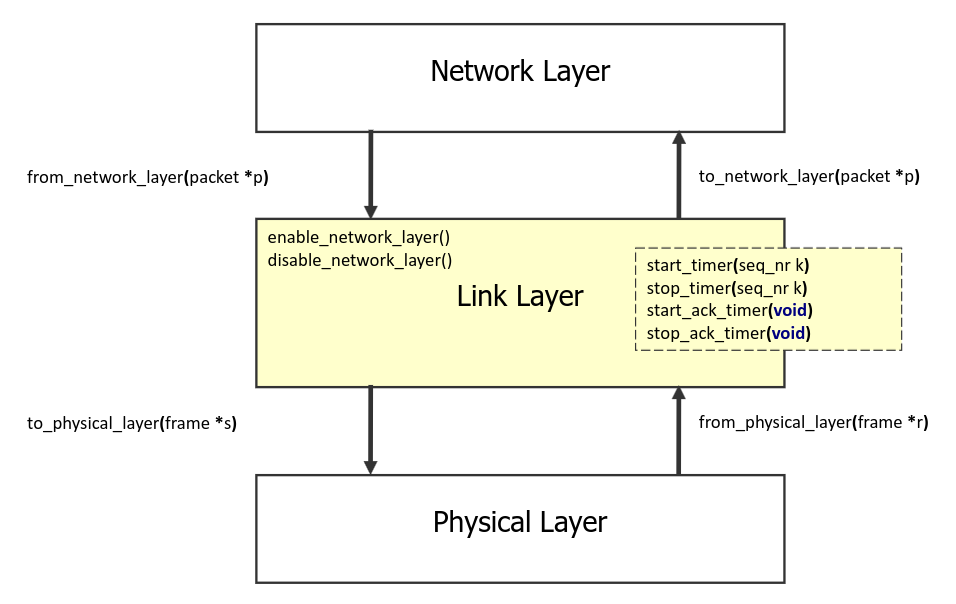
\includegraphics[scale=0.27]{interface}
\end{center}

\subsubsection{Simplex}
\begin{wrapfigure}[14]{r}{7cm}
	\begin{center}
		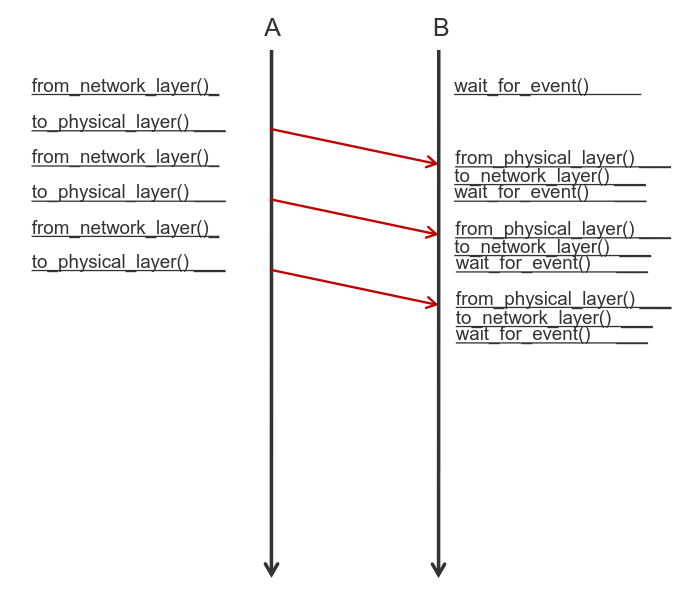
\includegraphics[width=7cm]{simplex}
	\end{center}
\end{wrapfigure}
This is the simplest mechanism of flow control: transmission happens in \textbf{one direction} without \textit{sequence number} or \textit{acknowledgment} and ignoring \textit{processing time}. The sender \textbf{fetches} and \textbf{sends} data in an infinite loop, while the receiver \textbf{gets} it and \textbf{forwards} it to the network layer.
While being extremely \textbf{simple}, it assumes that the channel never damages or loses frames and that the \textbf{network layer} is \textbf{always ready}.\\\\
To solve all of these problems we have two approaches:
\begin{itemize}
	\item \textbf{Feedback} based flow control: receiver sends information back to the sender allowing him to send more data
	\item \textbf{Rate} based flow control: protocols limits the data a sender may transmit without feedback from the receiver
\end{itemize}

\subsubsection{Stop-and-wait}
\begin{wrapfigure}[14]{r}{7cm}
	\vspace{-1cm}
	\begin{center}
		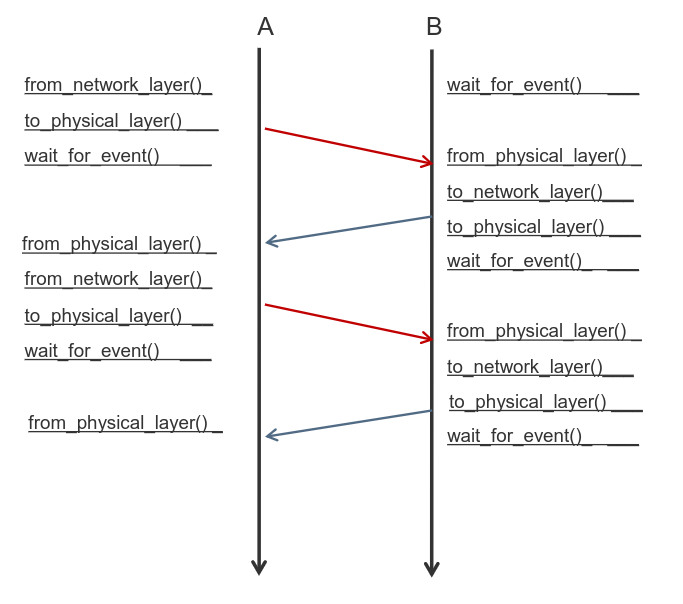
\includegraphics[width=7cm]{stopwait}
	\end{center}
\end{wrapfigure}
This approach uses a \textbf{bidirectional channel}: the sender sends a data blocks and waits until an \textbf{acknowledgment} from the receiver arrives or a \textbf{timeout} is reached. An unacknowledged data block is resent.\\\\
Since the channel is not error-free, we use the \textbf{Alternating Bit Protocol} to signal a duplicate data block by using one bit flag.\\\\
The main drawback is that there are large waiting periods between the transmissions, hence \textbf{capacity is wasted}.

\paragraph{Piggybacking}
To get a \textbf{full-duplex} communication we could use two simplex channels with \textbf{stop-and-wait}. That would be a waste of resource, hence the technique of \textbf{piggybacking}.\\
It consists of \textbf{stop-and-wait} on a single channel for both directions: data frames and ACK are intermixed and distinguished by the \textbf{Type} field in the header.\\
An even more efficient approach is to include the ACK message in header of the data frame. When a data packet arrives, the receiver waits a particular time interval to send the ACK back.

\begin{figure}[!h]
	\hfil
	\subfigure[Separate messages]{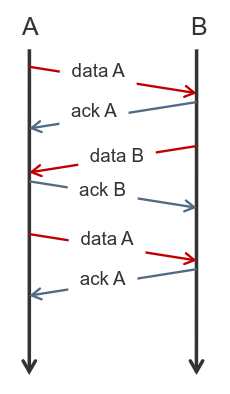
\includegraphics[scale=0.4]{ack1}}
	\hfil
	\subfigure[Single message]{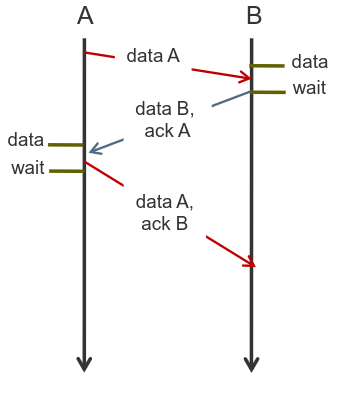
\includegraphics[scale=0.4]{ack2}}
\end{figure}

\subsubsection{Sliding window}
To avoid long waiting periods of the sender, both parts agree on a \textbf{transmission window} of size $W$. Any message sent in that window doesn't need a specific ACK, when ACK is sent all previous messages in the window are acknowledged.\\
For this technique, \textbf{sequence numbers} need to be introduced, to allow sequentially numbering of the messages. If coded on $n$bits, the sequence number $\text{seqnum} \in \{0, 1, \ldots, 2^n-1\}$ and \textbf{wraps around} the end.

\begin{note}
	All frames in the window must be \textbf{buffered}, hence for a window of size $W$ a buffer for $W$ frames is needed.
\end{note}

\begin{observation}
	It's important to have a window of size $W < 2^n$ and not $W \leq 2^n$ to avoid ambiguities.
\end{observation}

\paragraph{Pipelining}
Long round-trip time is an issue in terms of efficiency. If $\text{bandwidth} \cdot \text{round-trip-delay}$ is large, a big window is needed to fill the pipe capacity. Having a bigger window size means also having more bit-errors and packet loss.\newpage
\noindent There are three ways of handling the \textbf{pipelining}:
\begin{itemize}
	\item \textbf{Go-back-N}: each frame has an associated \textbf{timer} of the expected time to receive an ACK. When an ACK is received a new packet is sent and the buffer is updated (window slide). When the timer expires, the sender retransmits all buffered frames.
	\item \textbf{Selective repeat}: when a frame is correct, send ACK. When it's missing, \textbf{buffer} the following correct frames. When the missing message arrives, send ACK for that one and all the buffered frames. Capacity is used more efficiently but the receiver needs more buffer.
	\item \textbf{Selective reject}: works similar to selective repeat but when a frame is missing, a negative acknowledgment is sent and just that frame is repeated. A variation is to send a list of missing frames instead of a single NACK. This method enhances \textbf{efficiency} but it's more complex.
\end{itemize}

\begin{figure}[!h]
	\hfil
	\subfigure[Go-back-N]{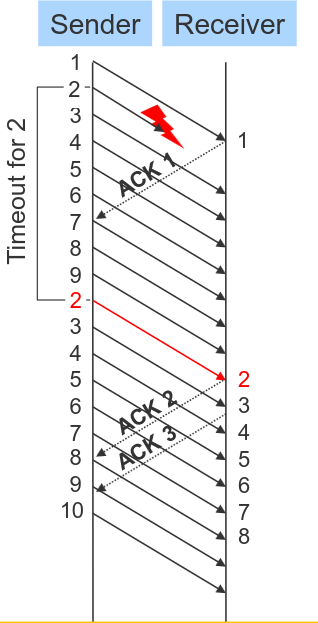
\includegraphics[scale=0.3]{gobackn}}
	\hfil
	\subfigure[Selective repeat]{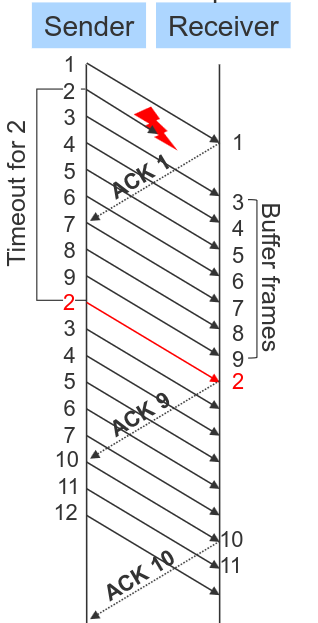
\includegraphics[scale=0.3]{srep}}
	\hfil
	\subfigure[Selective reject]{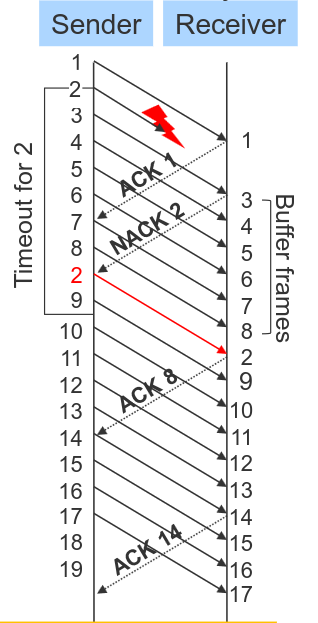
\includegraphics[scale=0.3]{srej}}
\end{figure}

\begin{note}
	Some protocols require many timers: implement them by using one hardware timer and store expiration times in a linked list that's updated during protocol runtime.
	\begin{center}
		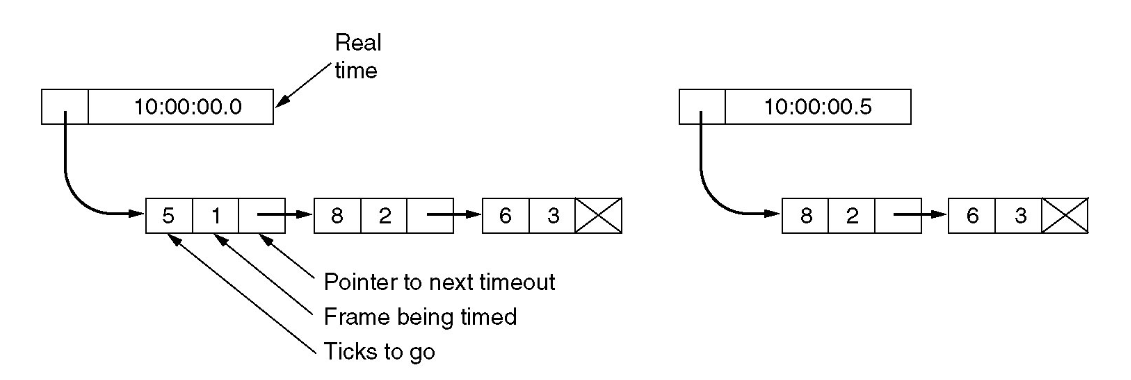
\includegraphics[scale=0.4]{timer}
	\end{center}
\end{note}

\newpage
\subsection{Medium Access Control}
When dealing with a medium shared by $n>2$ nodes, a NIC needs to manage:
\begin{itemize}
	\item \textbf{Channel allocation}: medium access control, organizes the order of transmitting nodes on the channel. There are two different approaches:
	\begin{itemize}
		\item \textbf{Distributed MAC}: there are $n$ nodes that generate frames for transmission on shared single channel. If two frames are transmitted simultaneously, the frames are lost. Time management can happen in two ways:
		\begin{itemize}
			\item \textbf{Continuous} time: no master clock, transmission of frames can begin at any time
			\item \textbf{Slotted} time: time is divided into discrete intervals (slot), frame transmission begins always at the start of a slot
		\end{itemize}
		\item \textbf{Centralized MAC}: a \textbf{master device} manages channel allocation
		\begin{itemize}
			\item \textbf{Round-Robin}: the master device polls each node periodically (fixed TDMA) and each node gets the entire transmission capacity for a fixed time interval
			\begin{center}
				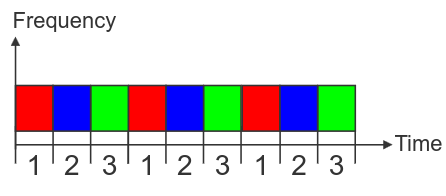
\includegraphics[scale=0.3]{ftdma}
			\end{center}
			\item \textbf{FDMA}: the master allocates a different frequency to each node, which gets a portion of the transmission capacity for the whole time
			\begin{center}
				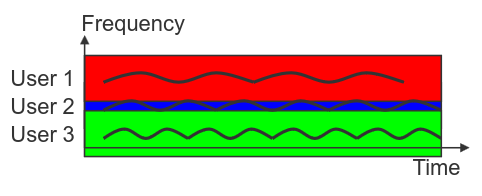
\includegraphics[scale=0.3]{fdma}
			\end{center}
		\end{itemize}
		Since users are typically \textbf{bursty}, most subchannels will be idle most of the time.
	\end{itemize}
	\item \textbf{Node identification}: addresses of the nodes on the medium, \textbf{MAC Addresses}, typically $6$bytes long in hexadecimal notation
\end{itemize}

\subsubsection{Token}
\begin{wrapfigure}[5]{r}{3cm}
	\vspace{-1.5cm}
	\begin{center}
		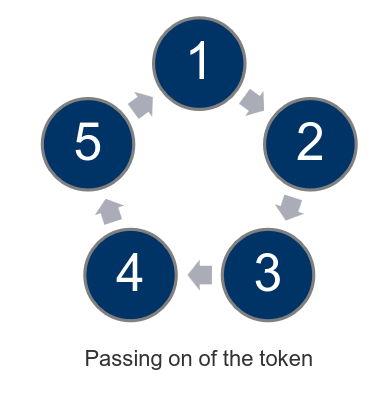
\includegraphics[width=3cm]{token}
	\end{center}
\end{wrapfigure}
Multiple access using a \textbf{token} (a bit sequence) means that only the owner of the token is allowed to send. The token is then passed between all the nodes. It's particularly suitable for a \textbf{ring} topology. It guarantees access without collisions, efficient and fair. It's very complex, e.g. when handling a lost token.

\subsubsection{ALOHA}
This multiple access technique was derived from the principles of \textit{ALOHANET}\footnote{Developed by Norman Abramson on the Hawaiian Islands in 1970s, a network connecting computers on islands over radio. There were two channels: uplink shared by nodes (collision may occur) and downlink used by main computer. The packets were ACKed by the main computer. Good performance only in low traffic.}. Nodes are \textbf{uncoordinated} and they can send at any time on every frequency. When several nodes are sending at the same time, a \textbf{collision} occurs: the frame are lost and each sender wait a \textbf{random time} to transmit again.

\begin{center}
	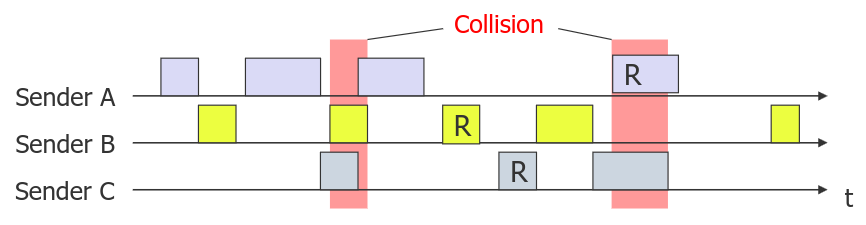
\includegraphics[scale=0.4]{aloha}
\end{center}

\paragraph{Slotted ALOHA} Even small overlaps would cause a collision, hence having a \textbf{low throughput} and no guaranteed response time. The improvement was \textbf{slotted} ALOHA: the time axis was divided into \textbf{time slots} and each sender could send at any time but only at the beginning of a time slot. This brought fewer collisions but now \textbf{synchronization} of the computers was needed.

\begin{center}
	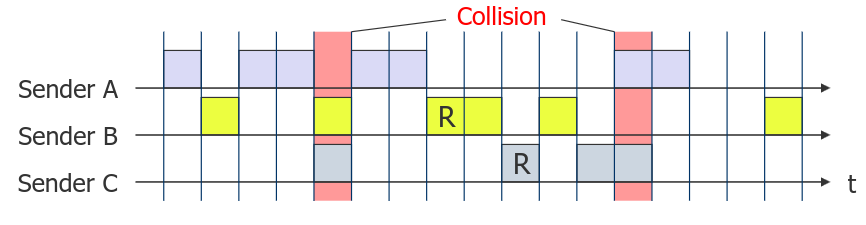
\includegraphics[scale=0.4]{slotaloha}
\end{center}

\paragraph{Performance}
Given an infinite number of users generating data, the transmissions (and retransmissions) are generated according to a Poisson distribution with intensity $\lambda$. Hence, the probability of $k$ transmission attempts in an interval $[0,t)$ is
\begin{equation*}
	P(X=k)=\frac{(\lambda t)^k}{k!}\cdot e^{-\lambda t}
\end{equation*}
The \textbf{throughput} $S$ is given by the load $G$ and the probability of a \textbf{successful} transmission $P_0$
\begin{equation*}
	S=G \cdot P_0
\end{equation*}
A frame is \textbf{successfully} transmitted if no other frames are within the \textbf{vulnerability period} $t$
\begin{equation*}
	P_0 = P(X=0)=\frac{(Gt)^0}{0!}\cdot e^{-Gt} = e^{-Gt}
\end{equation*}
Then, assuming that time unit is the time to send a single frame, we have:
\begin{itemize}
	\item \textbf{ALOHA} with vulnerability period of $2$
	\begin{equation*}
		S=G\cdot P_0 = G \cdot e^{-2G}
	\end{equation*}
	\item \textbf{Slotted ALOHA} with vulnerability period of $1$
	\begin{equation*}
		S=G\cdot P_0 = G \cdot e^{-G}
	\end{equation*}
\end{itemize}
\begin{center}
	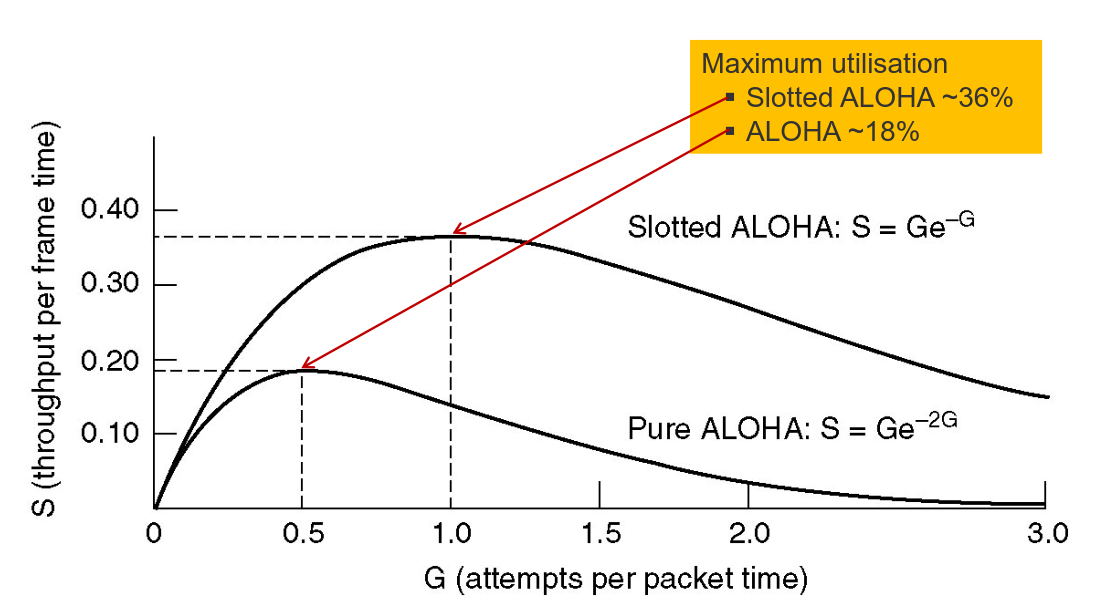
\includegraphics[scale=0.3]{alohaper}
\end{center}

\newpage
\subsubsection{CSMA}
Since ALOHA doesn't perform well under high loads, a solution is to reduce collisions: a sender first examines if another node is already transmitting and if nobody is currently sending, they are free to start. This is called \textbf{Carrier Sense Multiple Access} and it's a \textbf{simple} way with good utilization of the network. The main drawback is that there is \textbf{no guarantee} for the access to the medium. It only works with \textbf{short transmission delay}.\\
There are three variants:
\begin{itemize}
	\item \textbf{Non persistent}: when a node has data to send, it first listens to the channel. If it's busy, the computer listens and waits for availability. As soon as the channel is idle, the frame is transmitted. If a collision occurs, the node waits a random amount of time and starts again.
	\item \textbf{Persistent}: when a node has data to send, it first listens to the channel. If it's busy, the node waits a random amount of time and starts again. Else, it starts transmitting.
	\item $p$\textbf{-persistent}: if the channel is idle, a node that has data to send transmits with \textbf{probability} $p$ in current slot and defers until next slot with probability $(1-p)$ going then back to the beginning. If the channel is busy, the node waits from the next slot and goes back to the beginning. If a collision occurs, the node waits a random amount of time and goes back to the beginning. It's applicable in slotted time environments (slotted ALOHA).
\end{itemize}

\begin{center}
	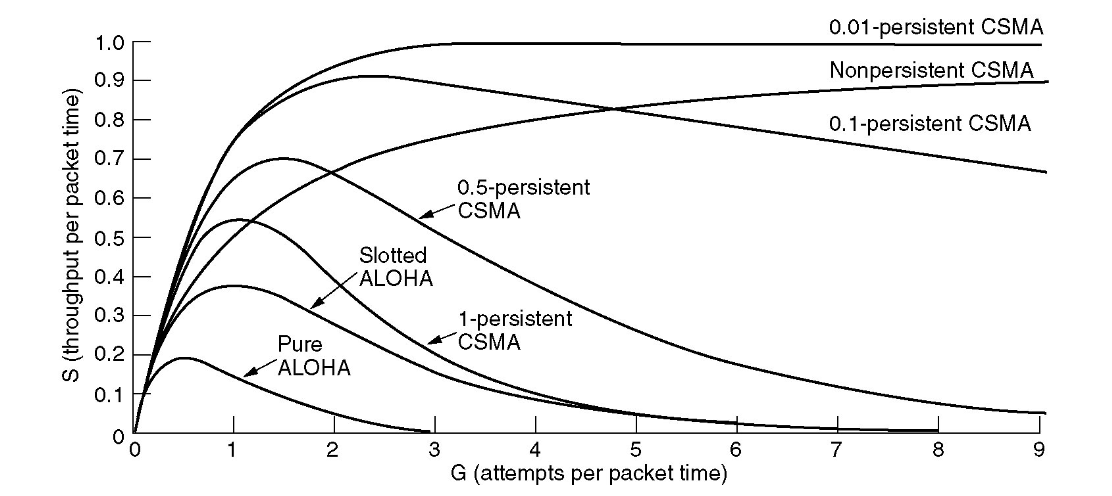
\includegraphics[scale=0.3]{csma}
\end{center}

\paragraph{CSMA/CD}
CSMA with \textbf{Collision Detection} aims to reduce the waste produced by collisions between long frames: the node listens through their own transmission, if what they hear is different from what they sent, stop the transmission and wait a random amount of time.
\begin{center}
	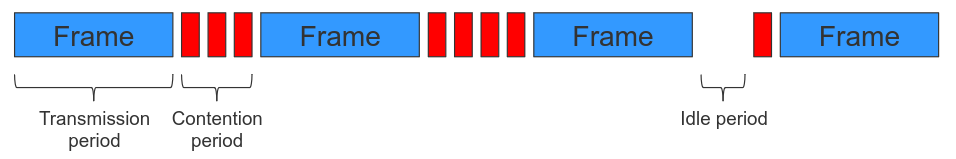
\includegraphics[scale=.3]{csmacd}
\end{center}

\subsubsection{Reservation mechanisms}
Reserve the channel to avoid collisions. Works in two \textbf{alternating phases}:
\begin{enumerate}
	\item \textbf{Reservation}: the sender makes a reservation by indicating the wish to send data (in some cases also the length)
	\item \textbf{Transmission}: if reservation is ok, the data communication takes place 
\end{enumerate}
It's very efficient in terms of capacity but there is more delay due to the reservation procedure.\\
The reservation can be:
\begin{itemize}
	\item \textbf{Centralized}: a master periodically queries all the nodes and checks if they have to send data, assigning sending rights
	\item \textbf{Distributed}
	\begin{itemize}
		\item \textit{Explicit}: \textbf{Bit-Map} approach, uses a small \textbf{reservation frame} in the first phase and a \textbf{data frame} of constant size in the second phase. There are two variants:
		\begin{itemize}
			\item \textbf{Without contention}: each user $i$ is assigned to the $i$th slot in the reservation frame. If it wants to send the data, it sets the bit to $1$. After the reservation phase, all nodes have set their bit and can send the data in the order of the bits in the frame
			\begin{center}
				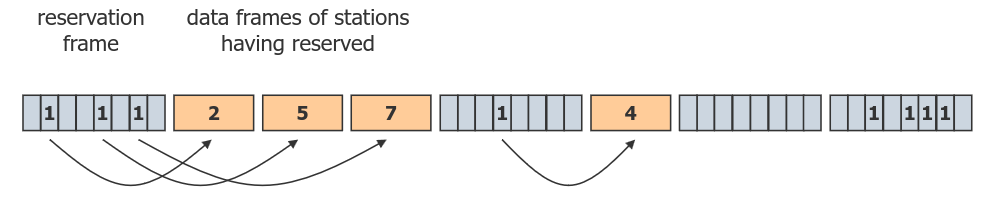
\includegraphics[scale=.3]{bitmap1}
			\end{center}
			\item \textbf{With contention}: the reservation frame consists of a limited number of contention slots  $<i$. Users try to get a random contention slot writing their computer ID into a slot. If there is no collision in the reservation phase, a node may send.
			\begin{center}
				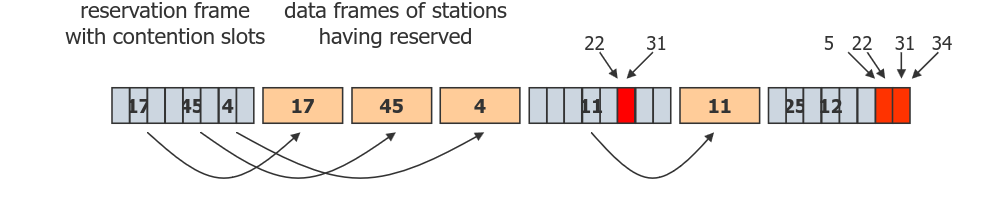
\includegraphics[scale=.3]{bitmap2}
			\end{center}
		\end{itemize}
		\item \textit{Implicit}
		\begin{itemize}
			\item \textbf{Binary Countdown}: there are priorities based on the ID of the computer. When nodes need to send data, they enter a \textbf{contention} phase where they broadcast their ID bit by bit. The smaller addresses give up.
			\item \textbf{Adaptive Tree Walk}: the nodes are the leaves of a binary tree. In the first contention slot following a successful frame (slot $0$), all nodes are allowed to try to acquire the channel. If there is a collision, only the nodes from the left subtree are allowed to try. If successful, the slot is reserved for the right subtree.
		\end{itemize}
	\end{itemize}
\end{itemize}

\subsection{Protocols}
\subsubsection{PPP}
\textbf{Point to Point Protocol} establishes a direct connection between two nodes. It supports synchronous and asynchronous connections. It uses:
\begin{itemize}
	\item Specified \textbf{frame format} with \textbf{error detection}
	\item \textbf{Sliding window} approach for flow control
	\item Specified connection establishment and tear down
\end{itemize}
It doesn't use medium access control since there is no need to on point-to-point links.
\paragraph{Connection} The connection happens in three steps:
\begin{enumerate}
	\item PPP establishes a \textbf{basic physical layer connection}, testing that the layer is ready
	\item \textbf{Link Control Protocol} configures the NIC on each end of the link:
	\begin{itemize}
		\item \textit{Maximum Frame Size} (MTU)
		\item \textit{Escape characters}
		\item \textit{Magic numbers}: identifying an end or to detect looped links
		\item \textit{Authentication method}
	\end{itemize}
	It also manages the \textbf{termination} of the link layer connection.
	\newpage
	The \textbf{frame types} are defined between the \textit{initiator} and the \textit{responder} as follows:
	\begin{table}[!h]
		\centering
		\begin{tabular}{|c|c|c|}
			\hline
			\textbf{Name} & \textbf{Direction} & \textbf{Description}\\
			\hline
			\textit{configure-request} & $I \to R$ & List of proposed options and values \\
			\hline
			\textit{configure-ack} & $I \leftarrow R$ & All options are accepted \\
			\hline
			\textit{configure-nack}& $I \leftarrow R$ & Some options are not accepted \\
			\hline
			\textit{configure-reject} & $I \leftarrow R$ & Some options are non negotiable \\
			\hline
			\textit{terminate-request} & $I \to R$ & Request to shut the line down \\
			\hline
			\textit{terminate-ack} & $I \leftarrow R$ & OK, line shutdown \\
			\hline
			\textit{code-reject} & $I \leftarrow R$ & Unknown request received \\
			\hline
			\textit{protocol-reject} & $I \leftarrow R$ & Unknown protocol requested \\
			\hline
			\textit{echo-request} & $I \to R$ & Send this frame back \\
			\hline
			\textit{echo-reply} & $I \leftarrow R$ & Here is the frame back \\
			\hline
			\textit{discard-request} & $I \to R$ & Just discard this frame (testing)\\
			\hline
		\end{tabular}
	\end{table}
	\item \textbf{Network Control Protocol} negotiates the network layer conditions (e.g. Internet Protocol Control Protocol configures IPv4 networks address or compression options) and manages the tear down of the network layer connection (frees IP)
\end{enumerate}

\begin{center}
	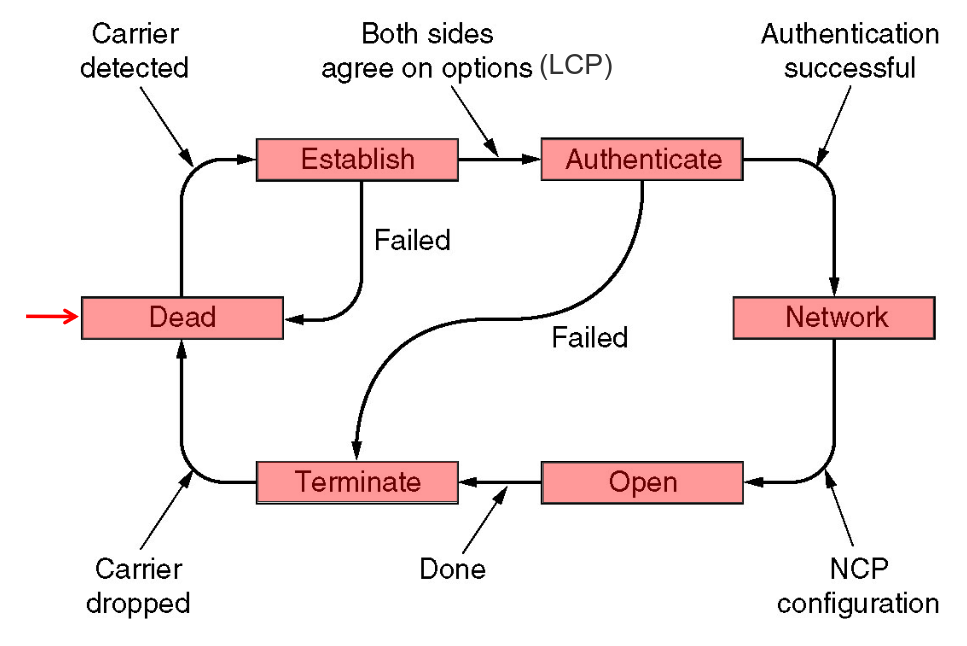
\includegraphics[scale=.25]{pppstates}
\end{center}
PPP is \textbf{character oriented} (byte oriented) and uses \textbf{byte stuffing}.
\begin{center}
	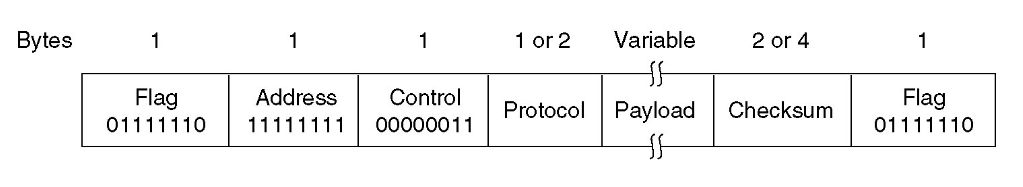
\includegraphics[scale=0.4]{ppp}
\end{center}
\begin{itemize}
	\item \textbf{Flag}: start of frame with special flag $01111110$ while end of frame is omitted for successive frames
	\item \textbf{Address}: useless, inherited from HDLC, it's set to $11111111$
	\item \textbf{Control}: set to \textbf{unnumbered mode} $00000011$, meaning without sequence numbering and acknowledgments
	\item \textbf{Protocol}: specifies to which network layer the payload should be delivered. For IP it's $00000110$
	\item \textbf{Checksum}: just \textbf{detection}, default is $16$ bit CRC with generator polynomial $x^{16}+x^{12}+x^5+1$ computed over \textit{Address}, \textit{Control}, \textit{Protocol}, \textit{Payload} and \textit{Padding}
\end{itemize}

\paragraph{Usage} PPP used to be the default link layer protocol for \textbf{dial-up} internet access. Now it's still used on \textbf{point-to-point optical links} (PPPoE) and for the last mile with DSL (PPPoA).

\subsubsection{Ethernet}
\paragraph{History} After ALOHA, Xerox began experimentation on network over \textbf{coaxial} cables. In 1976 Robert Metcalf created Ethernet, an improvement over ALOHA  with CSMA/CD. Between 1978 and 1983 the new standard IEEE 802.3 was created.\\
Initially it was a network over a \textbf{bus} topology: it was hard to maintain and debug if the bus got damaged. The solution was to implement a \textbf{star} topology where the cable goes through a central point: initially a \textbf{hub} (just a repeater, still CSMA/CD) and later a \textbf{switch} (one NIC per interface, no need of CSMA/CD).

\paragraph{Frame}
\begin{center}
	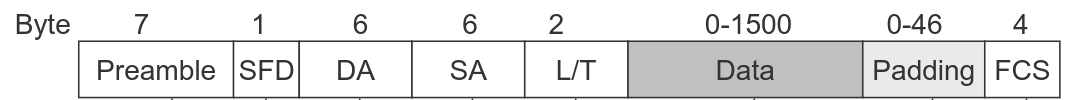
\includegraphics[scale=.3]{ethframe}
\end{center}
\begin{itemize}
	\item \textbf{Preamble}: 7 bytes, each one $10101010$, flag for synchronization
	\item \textbf{Start Frame Delimiter}: one byte $10101011$ marking the beginning of the frame
	\item \textbf{Destination address}: $6$ bytes containing the MAC address of the receiver
	\item \textbf{Source Address}: $6$ bytes containing the MAC address of the sender
	\item Depending on the version
	\begin{itemize}
		\item \textbf{Data length} in 802.3, ranging from $0$ to $1500$
		\item Identification of the \textbf{upper layer protocol} in Ethernet II
	\end{itemize}
	\item \textbf{Data}
	\item From $0$ to $46$ bytes of \textbf{padding} to fill up the frame to at least $64$ bytes, otherwise small fragments are discarded
	\item \textbf{Frame Check Sequence}: $4$ bytes that uses a $32$bit CRC computed over \textit{DA}, \textit{SA}, \textit{length}/\textit{type},\textit{data} and \textit{padding}
\end{itemize}

\paragraph{MAC Address}
\begin{wrapfigure}[5]{r}{6cm}
	\vspace{-.5cm}
	\begin{center}
		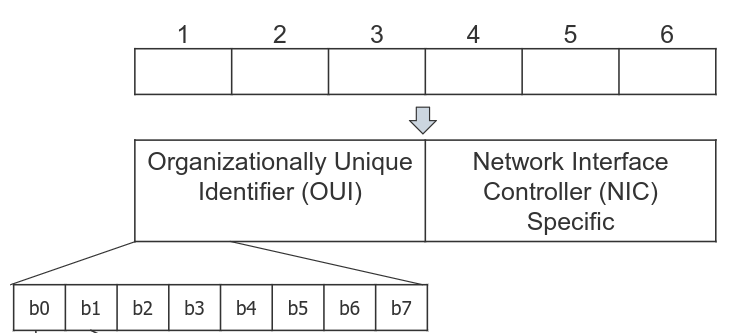
\includegraphics[width=6cm]{mac}
	\end{center}
\end{wrapfigure}
The MAC address is a $6$ bytes long number assigned uniquely by IEEE and locally administered. It can be:
\begin{itemize}
	\item \textbf{Unicast}, starting with $0$
	\item \textbf{Multicast}, starting with $1$
	\item \textbf{Broadcast} with all $1$
\end{itemize}

\paragraph{Multiple Access Control} Ethernet collision resolution mechanism is based on CSMA/CD: listen before sending and stop as soon as simultaneous transmissions are detected. A simple solution but with a possible large delay before sending.\\\\
The waiting period after a collision needs to be kept small to avoid long delays but at the same time that makes the risk of subsequent conflict higher. The solution is \textbf{Binary Exponential Backoff}: the random waiting period is drawn from an \textbf{increasing interval}. After $i$ collisions the node waits drawing a random number between $[0, 2^i-1]$, after $10$ collisions the interval becomes $0, 2^{10}-1$ and after $16$ the node gives up.\\\\
When the channel is free again the node waits $x$ time slots before starting again, where a \textbf{time slot} corresponds to the minimum Ethernet frame length.\\\\
The major drawback is that it tends to prefer last contention winners and new contending nodes over the others, being \textbf{unfair}.

\begin{observation}[Collision detection]
	Since the propagation speed is \textbf{finite}, collision detection is not instantaneous. The solution is to adjust \textbf{minimum packet length} and \textbf{maximum traveled distance}. A node needs to be sure that the beginning of its message reached the receiver before assuming there  was no collision and stops listening.
\end{observation}

\paragraph{Physical layer} The physical layer used with Ethernet is \textbf{baseband} encoding with \textbf{Manchester Encoding}. The voltages used are $\pm 0.85V$.

\paragraph{Standards} Some Ethernet standards are:
\begin{itemize}
	\item \textbf{10Base-2} (cheapnet): cheap coaxial cable. Terminals are attached with BNC connectors, maximum $5$ segments, $30$ nodes per segment, at least $0.5m$ between each node, $185m$ maximum segment length and a maximum expansion of $925m$
	\item \textbf{10Base-T} (twisted pair): star topology using twisted pair where several nodes are connected through a hub. Devices are attached with a RJ45 plug where 2 out of 4 cables are used. Maximum cable length to the hub is $100m$ and maximum extension $200m$
	\item \textbf{10Base-F}: Ethernet with fiber optics, expensive but excellent against noise. Used to connect distant buildings
	\item \textbf{Fast Ethernet}: concept based on \textit{10Base-T} with a central hub or switch. $100$Mbps transmission rate. The speed was a problem for the collision detection, hence the maximum distance was reduced to $200$m. It also brought \textbf{auto-configuration} of NICs (speed and communication mode)
	\begin{itemize}
		\item \textbf{100Base-T4}: UTP cable CAT3, using all the 4 cables pairs, and 8B6T encoding
		\item \textbf{100Base-TX}: UTP cable CAT5, using only 2 cable pairs, and 4B5B encoding
		\item \textbf{100Base-FX}: optical fiber, one per direction, with a maximum cable length to the hub of $400$m. There is a variant where only switches are allowed and the maximum length is $2$Km
	\end{itemize}
	\item \textbf{Gigabit Ethernet}: to avoid reducing the cable length while maintaining a high speed, a new minimum frame length of $512$ bytes was specified. The \textbf{Carrier Extension} was made through a \textit{nodata} field after the FCS. This field is added by the hardware while the software is kept unaware.
	\begin{center}
		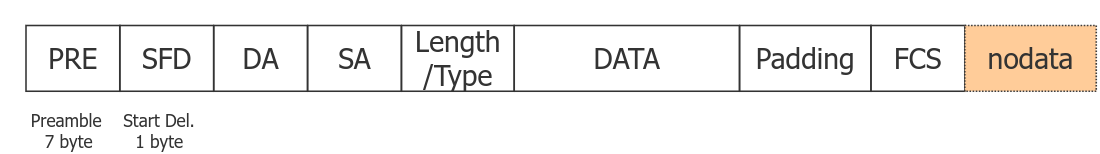
\includegraphics[scale=.2]{giga}
	\end{center}
	Now the sending of several successive frames (\textbf{Frame Bursts}) is possible without the need of repeated CSMA/CD: the sending MAC fills the gaps between the frames with \textbf{Interframe-Bits} (IFG), signaling to other nodes that the medium is still occupied.
	\begin{center}
		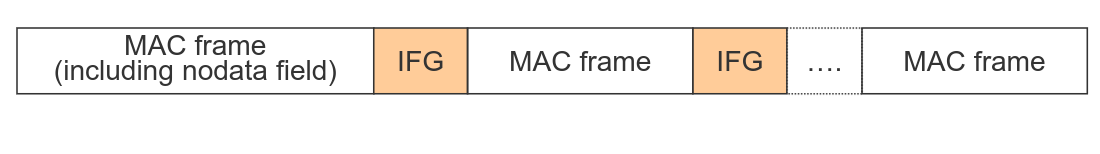
\includegraphics[scale=.2]{giga2}
	\end{center}
	\begin{itemize}
		\item \textbf{1000Base-T}: UTP cable CAT5/6/7, uses 4 pairs, maximum segment length of $100$m
		\item \textbf{1000Base-CX}: STP cable, uses 2 pairs, maximum segment length of $25$m
		\item \textbf{1000Base-SX}: multimode fiber with a maximum length of $550$m and on the $850$nm band
		\item \textbf{1000Base-LX}: single or multimode fiber over $5000$m and on $1300$nm band
	\end{itemize}
	\item \textbf{10-Gigabit Ethernet}: star topology using switch and optical fibers. CSMA/CD is no longer used since collisions cannot occur. There are two specifications on the physical layer:
	\begin{itemize}
		\item \textbf{LAN} with $10$Gbps
		\item \textbf{WAN} with $9.6215$Gbps for compatibility with SDH/SONET
	\end{itemize}
	The \textbf{copper} variants are:
	\begin{itemize}
		\item \textbf{10GBase-CX4}: four pairs of coaxial cables for each direction, maximum length of $15$m
		\item \textbf{10GBase-T}: either CAT6 ($50$m) or CAT7 ($100m$) cables, uses all the pairs in both directions in parallel, there is a filter for each cable to separate the sending and the receiving. On the physical layer a variant of \textbf{Pulse Amplitude Modulation} is used, with $16$ discrete levels between $\pm 1V$
	\end{itemize}
	The \textbf{fiber} variants are:
	\begin{table}[!h]
		\centering
		\begin{tabular}{|c|c|c|c|c|c|c|}
			\hline
			\textbf{Name} & \textbf{Type} & \textbf{Wavelength (nm)} & \textbf{PHY} & \textbf{Coding} & \textbf{Fiber} & \textbf{Range(m)} \\
			\hline
			\textit{10Base-SR} & Serial\footnotemark& $850$ & LAN & 64B66B & Multimode & $26-400$\\
			\hline
			\textit{10Base-LR} & Serial & $310$ & LAN & 64B66B & Singlemode & $10.000$\\
			\hline
			\textit{10Base-ER} & Serial & $1550$ & LAN & 64B66B & Singlemode & $40.000$\\
			\hline
			\textit{10Base-LX4} & WDM\footnotemark& $1275, 1300, 1325, 1350$ & LAN & 8B10B & Both & $10.000$\\
			\hline
			\textit{10Base-SW} & Serial & $850$ & WAN & 64B66B & Multimode & $26-65$\\
			\hline
			\textit{10Base-LW} & Serial & $1310$ & WAN& 64B66B & Singlemode & $10.000$\\
			\hline
			\textit{10Base-EW} & Serial & $1550$ & WAN& 64B66B & Singlemode & $40.000$\\
			\hline
		\end{tabular}
	\end{table}
\end{itemize}
\footnotetext{Only one transmission at a time.}
\footnotetext{Wavelength Division Multiplexing: several transmissions in parallel.} 

\paragraph{Logical Link Control} LLC interfaces with the network layer to provide:\\
\begin{wrapfigure}[5]{r}{5cm}
	\begin{center}
		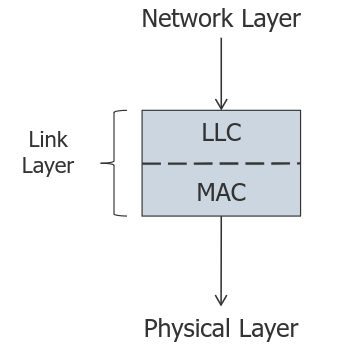
\includegraphics[width=5cm]{llc}
	\end{center}
\end{wrapfigure}
\begin{itemize}
	\item \textbf{Unreliable} datagram service
	\item \textbf{Acknowledged} datagram service
	\item \textbf{Reliable connection-oriented} service
\end{itemize}
The header contains:
\begin{itemize}
	\item \textbf{Destination} access point: which process to deliver
	\item \textbf{Source} access point
	\item \textbf{Control} field for sequence and ack numbers
\end{itemize}
Today it's \textbf{disbanded}.

\subsection{Infrastructure}
Different devices are used in different layers of a network.
\begin{center}
	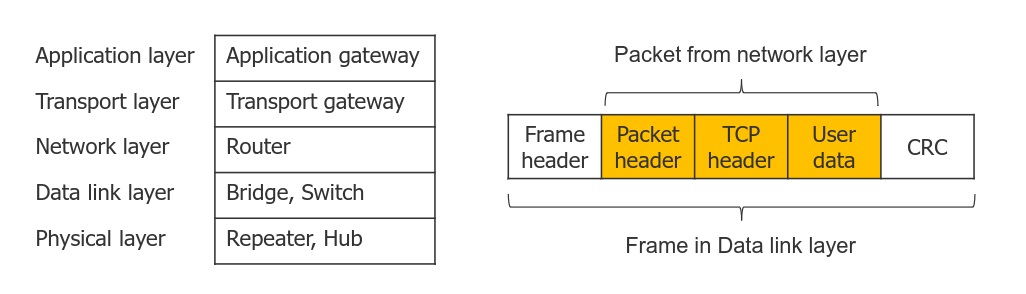
\includegraphics[scale=0.4]{infrastructure}
\end{center}

\newpage
\subsubsection{Physical elements}
\paragraph{Hub and Repeaters} A \textbf{Hub} sends the received packets on one side to all of the devices on the other side. A \textbf{repeater} links two different networks. Both of them do not understand packets, frames or headers: they just refresh the signal and \textbf{increase} the network \textbf{range}. They offer one channel shared between all nodes, a low cost but also low security solution.
\begin{figure}[!h]
	\hfil
	\subfigure[Hub]{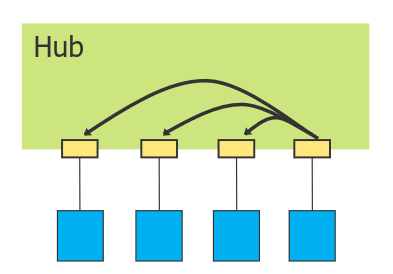
\includegraphics[scale=0.3]{hub}}
	\hfil
	\subfigure[Repeater]{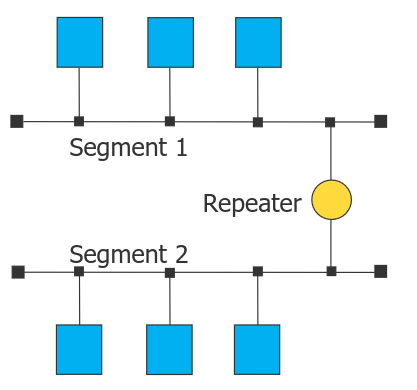
\includegraphics[scale=0.3]{repeater}}
\end{figure}

\paragraph{Bridging} Since many LAN exists due to load management reasons, security reasons and maximum length reasons, it's fundamental to connect them. A bridge should be \textbf{transparent} (different formats, data rates, lengths) and \textbf{flexible} (moving a node between networks should not require new HW or SW).\\
A bridge operates at the link layer, it processes frame addresses and supports different network types.

\begin{center}
	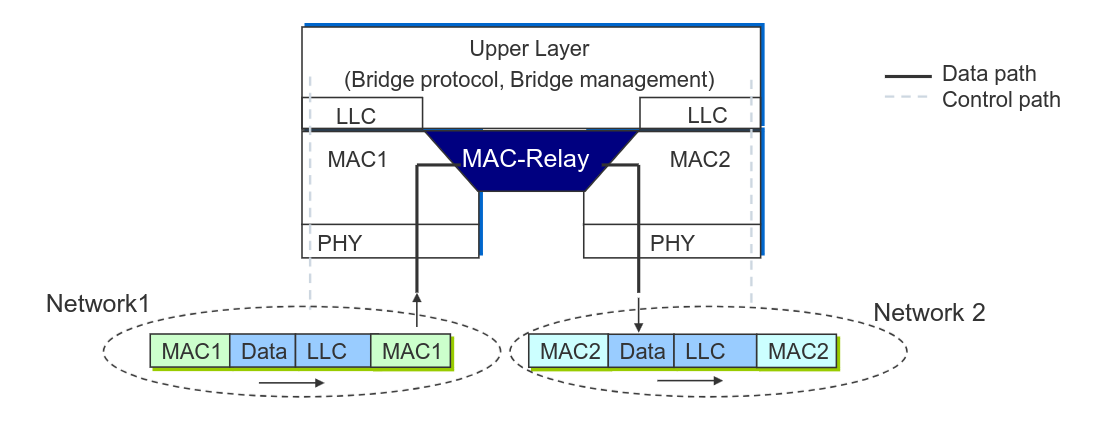
\includegraphics[scale=.3]{bridge}
\end{center}

\noindent Each bridge has a \textbf{forwarding database} with at least two entries. Each entry has:
\begin{itemize}
	\item \textbf{MAC Address}: host ID
	\item \textbf{Port}: port number of the bridge used to send data to the host
	\item \textbf{Age}: aging time of entry (optional)
\end{itemize}
The source field of a frame that arrives on a port tells which hosts are reachable from this port. For each frame received the bridge stores the source field in the database together with the port where the frame was received. All entries are deleted after a certain amount of time.

\subparagraph{Spanning Tree Protocol} Adding redundancy in a network will introduce \textbf{endless loops}. The idea behind a Spanning Tree is to relay frames only along the edges of a tree structure. It works as follows:
\begin{itemize}
	\item At the beginning each bridge assumes to be root and floods a packet containing its ID and current cost initialized at $0$ over all of its ports
	\begin{center}
		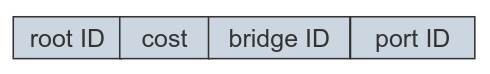
\includegraphics[scale=.3]{stp}
	\end{center}
	\item A bridge that receives such packet checks the root ID and compares it with its own. Both the ID and the costs are updated (its own cost for the sender bridge is summed with current cost value) for receiving packets with smaller ID and forwarded
	\item When the updated packets of all bridges have passed all other, there is an agreement on the \textbf{root bridge}. The received packets containing the smallest costs determine the \textbf{designated bridge} for a LAN and designated ports for the bridges to send out data
\end{itemize}

\paragraph{Switches}
\begin{wrapfigure}[15]{r}{5cm}
	\vspace{-0.5cm}
	\begin{center}
		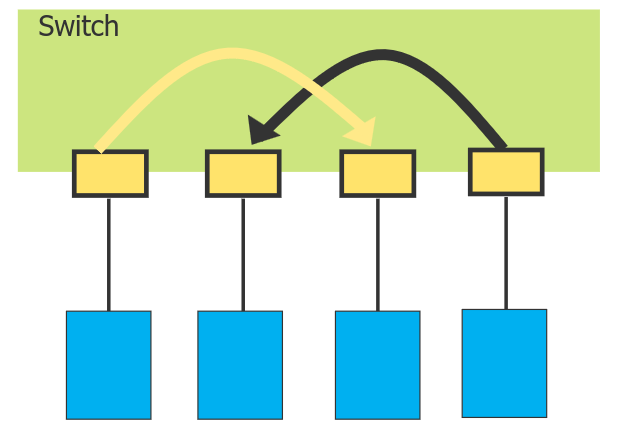
\includegraphics[width=4cm]{switch}
		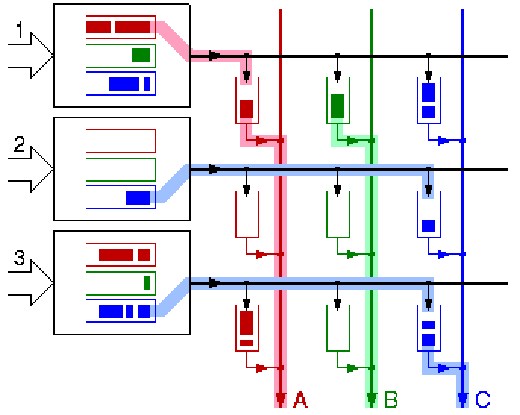
\includegraphics[width=4cm]{switchhw}
	\end{center}
\end{wrapfigure}
They are similar to bridges, except they have \textbf{point-to-point} NICs on each port. They have a \textbf{buffer} for each node/port and connected nodes can send and receive at the same time. There are also layer 3 and 4 switches with corresponding layer functionalities.\\\\
The most used HW implementation is \textbf{buffered crossbar}: for each input port provide buffers for the output ports. At any time only one input port can be connected to an output line. Collisions are almost impossible.


\paragraph{Routers} Since bridges uses non-scalable addresses, they are limit with the number of supported nodes. Moreover, they pass broadcast frames on every port, causing \textbf{broadcast storms} and do not communicate with hosts to hand over information on errors.\\\\
Routers, on the other hand, work on the Network layer: packets are forwarded towards destination based on a \textbf{global address}, hence overcoming the restriction on nodes number. Moreover they do not let broadcast through and improve performances by communicating with hosts.
\begin{center}
	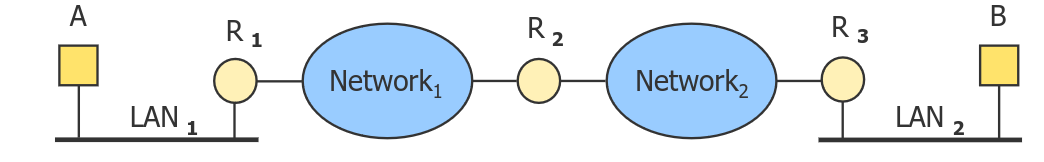
\includegraphics[scale=.3]{router}
\end{center}

\paragraph{Gateways} There are two types:
\begin{itemize}
	\item \textbf{Transport} layer: connect computers using different transport protocols, e.g. TCP/IP to ATM
	\item \textbf{Application} layer: understand the format and contents of the data and translate the message, e.g. email to SMS
\end{itemize}

\paragraph{Structured cabling} The idea is to \textbf{partition} a network through its cable infrastructure, which is connected to a \textbf{backbone} or a central switch. Each user outlet is cabled to a communication closet with an individual cable. In there, the user outlets terminate on \textbf{path panels}, usually mounted on $19"$ racks.\\
The \textbf{advantages} are:
\begin{itemize}
	\item \textbf{Consistency}: usage of the same cabling systems for data, voice and video
	\item Support \textbf{multi-vendor} equipment
	\item \textbf{Simple modifications}: support the changes in within the system (e.g. adding, changing, moving)
	\item \textbf{Simple troubleshooting}: problems are less likely to down the entire network and simplify the isolation and fixing of problems
	\item \textbf{Fault isolation}: by dividing the entire infrastructure into simple management blocks, it's easy to test and isolate specific points of fault and correct them
\end{itemize}

\subsubsection{VLAN}
While initially computers of an enterprise network were on a single LAN, today there are several because of new cabling technologies and security/load management necessities.\\
\textbf{Virtual LANs} allow the configuration on LANs \textbf{logically} instead of physically, provided that there is a \textbf{decoupling} between the two topologies.
\begin{figure}[!h]
	\hfil
	\subfigure[Physical topology]{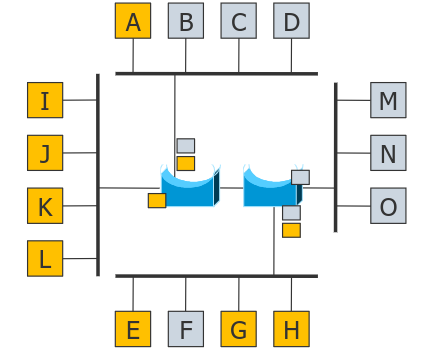
\includegraphics[scale=0.4]{swph}}
	\hfil
	\subfigure[Logical topology]{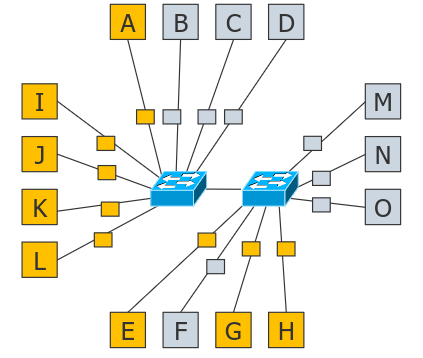
\includegraphics[scale=0.4]{swlog}}
\end{figure}
\newline VLAN-aware devices are needed, such as switches that have a table which tells which VLAN is accessible via which port. There are three possibilities:
\begin{itemize}
	\item Assign each port of the device to a VLAN-ID, allowing only the devices with that ID to attach to it
	\item Each MAC address is assigned to a VLAN, having a table that keep tracks of that
	\item Each Layer 3 protocol (IP address) is assigned to a VLAN but violating the layer independence
\end{itemize}
\textbf{IEEE 802.1Q} specifies a field in the frame header telling the VLAN assignment. The first VLAN-aware device adds the TAG based on the MAC address while the last one removes it. Newer NICs support this.
\begin{center}
	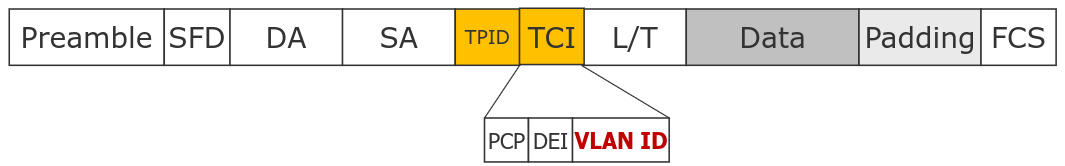
\includegraphics[scale=.3]{vlan}
\end{center}
The new fields are:
\begin{itemize}
	\item \textbf{Tag Protocol Identifier} ($0x8100$): serves as flag to differentiate with beginning of L/T field in a non-VLAN frame
	\item \textbf{Tag Control Information}
	\begin{itemize}
		\item \textbf{Priority Code Point}: 3bit priority field, refers to 802.1p
		\item \textbf{Drop Eligible Indicator}: indicates frames that can be dropped in case of congestion
		\item \textbf{VLAN Identifier}: 12bit VLAN-ID, between $0$ and $4095$
	\end{itemize}
\end{itemize}
\begin{note}
	\textbf{802.1ad}, then improved by 802.1ah, allows nested VLAN tags for bridging VLANs over providers.
\end{note}

\newpage
\subsubsection{Optical Transport Networks}
OTN creates an optical virtual private network by encapsulating data frames meaning multiple data sources can use the same channel. It replaced SDH/Sonet systems with the standards \textbf{G.709}, \textbf{G.798} and later. Supports the encapsulation of different protocols (e.g. IP, Ethernet frames) and both variable and constant bit rates.

\begin{center}
	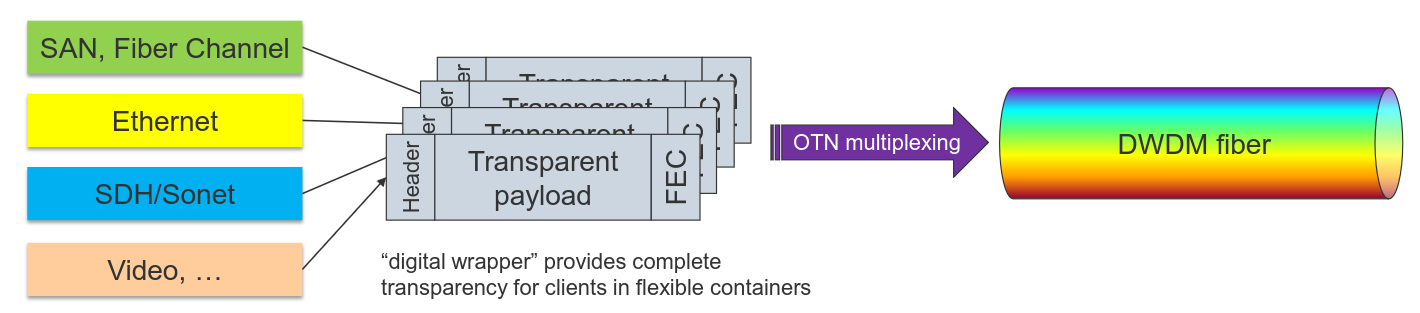
\includegraphics[scale=.3]{otn}
\end{center}